
% File acl2020.tex
%
%% Based on the style files for ACL 2020, which were
%% Based on the style files for ACL 2018, NAACL 2018/19, which were
%% Based on the style files for ACL-2015, with some improvements
%  taken from the NAACL-2016 style
%% Based on the style files for ACL-2014, which were, in turn,
%% based on ACL-2013, ACL-2012, ACL-2011, ACL-2010, ACL-IJCNLP-2009,
%% EACL-2009, IJCNLP-2008...
%% Based on the style files for EACL 2006 by 
%%e.agirre@ehu.es or Sergi.Balari@uab.es
%% and that of ACL 08 by Joakim Nivre and Noah Smith

\documentclass[11pt,a4paper]{article}
\usepackage[hyperref]{acl2020}
\usepackage{times}
\usepackage{graphicx}
\usepackage{latexsym}
\usepackage{float}
\usepackage{placeins}
\usepackage{booktabs}
\renewcommand{\UrlFont}{\ttfamily\small}

% This is not strictly necessary, and may be commented out,
% but it will improve the layout of the manuscript,
% and will typically save some space.
\usepackage{microtype}

\aclfinalcopy % Uncomment this line for the final submission
%\def\aclpaperid{***} %  Enter the acl Paper ID here

%\setlength\titlebox{5cm}
% You can expand the titlebox if you need extra space
% to show all the authors. Please do not make the titlebox
% smaller than 5cm (the original size); we will check this
% in the camera-ready version and ask you to change it back.

\newcommand\BibTeX{B\textsc{ib}\TeX}

%%%%%%%%%%%%%%%%%%%%%%%%%%%%%%%%%%%%%%%%%%%%%%%%%%%%

\title{Hw2: Language Modeling across Domains with Various Smoothing Methods}

\author{Sam Showalter \\
  University of California, Irvine \ (showalte) \\  
\texttt{showalte@uci.edu}} 

\date{}

%%%%%%%%%%%%%%%%%%%%%%%%%%%%%%%%%%%%%%%%%%%%%%%%%%%%

\begin{document}
\maketitle
\begin{abstract} 
  Language modeling has been prominent in natural language processing (NLP) for
  decades and takes in roots in probabilistic modeling. 
  However, modeling long-range dependencies with n-gram models explicitly is intractable since
  larger contexts become less and less likely to be observed in data. In turn, n-grams rely on Markovian assumptions;
  conditioning on the previous n-words in a context is considered a sufficient statistic of future likelihood. This homework 
  explores language modeling across three corpuses from different timeframes and domains. Several
  methods of probability smoothing are applied to these models to improve generalization, including Laplacian, add-k
  , and stupid backoff \cite{brants2007large} smoothing. 

  Our findings indicate that across all corpuses, stupid backoff smoothing was most effective at ensuring generalization for n-grams. Moreover, 
  bigram models were best suited for generalizing across all corpuses, though for more homogenous corpuses ( \texttt{reuters}, \texttt{gutenberg})
  benefitted from additional context via higher order n-grams (namely, trigrams).

  We also applied our tuned n-gram models for each corpus across domains. Using the same set of basic 
  prefixes, we compared generated sentences between these models as well as perplexity scoring.
  Our high level observations include that the \texttt{brown} and \texttt{gutenberg} corpuses were most similar lexically, and that
  the \texttt{brown} corpus appeared to be most diverse. In general, natural sounding sentences scored lower perplexities on 
  n-gram models with $ n > 1$, but with poetic or syntactically jumbled sentences, unigram models scored lower values. Due to the length of 
  some generated sentences, extra information is stored in the Appendix \ref{appendix}. 
\end{abstract}


%%%%%%%%%%%%%%%%%%%%%%%%%%%%%%%%%%%%%%%%%%%%%%%%%%%%
% Introduction
%%%%%%%%%%%%%%%%%%%%%%%%%%%%%%%%%%%%%%%%%%%%%%%%%%%%
\section{Related Work: Language Model Implementations}

Language modeling addresses the challenge of generating predictions from sparse data. Language in any
dialect is diverse, ambiguous, and generally full of syntax flexibility. As a result, effective methods 
tend to make use of intelligent forms of probability smoothing \cite{chen1999empirical}.
Without probabilistic smoothing, n-gram models will see certain vocabulary combinations as impossible \cite{jelinek1980interpolated} and be
infinitely surprised when a combination of tokens not witnessed during training is observed at test time.

In addition, language model capacity is heavily influenced by their n-gram cardinality. Trigram models
tend to incorporate higher capacity than bigram models, and so on. Our hyperparameter tuning also focuses on 
identifying the optimal n-gram cardinality for generalization as well as the correct regularization to assist
in the prevention of overfitting.


%%%%%%%%%%%%%%%%%%%%%%%%%%%%%%%%%%%%%%%%%%%%%%%%%%%%
% Experimental setup
%%%%%%%%%%%%%%%%%%%%%%%%%%%%%%%%%%%%%%%%%%%%%%%%%%%%
\section{Experimental Setup}%
\label{sec:experimental_setup}

Our language model was implemented from scratch and is defined by the following 
characteristics. 
\begin{enumerate}
  \item Our package can accomodate an arbitrary context ($n$) and
    produces padding when necessary for modeling short phrases with the token 
    immediately preceding sentence start represented as \texttt{SOS} and, as necessary,
    \texttt{padding} tokens placed before it.
  \item Our package can implement arbitary add-k smoothing (including Laplacian) as well as
    stupid backoff smoothing.
  \item No centralization of tokens with low counts into \texttt{Unk} tokens is undertaken.
    We made this design choice in an effort to reasonably
    model rare tokens without excluding them entirely.
\end{enumerate}

With this language model package, we implemented three rounds of hyperparameters tuning. First,
we explore the performance of different add-k smoothing methods on the bigram model. Using the results
of this ablation, we examine the impact 
%%%%%%%%%%%%%%%%%%%%%%%%%%%%%%%%%%%%%%%%%%%%%%%%%%%%
% Smoothing exploration
%%%%%%%%%%%%%%%%%%%%%%%%%%%%%%%%%%%%%%%%%%%%%%%%%%%%
\FloatBarrier
\begin{figure*}[htpb]
  \centering
  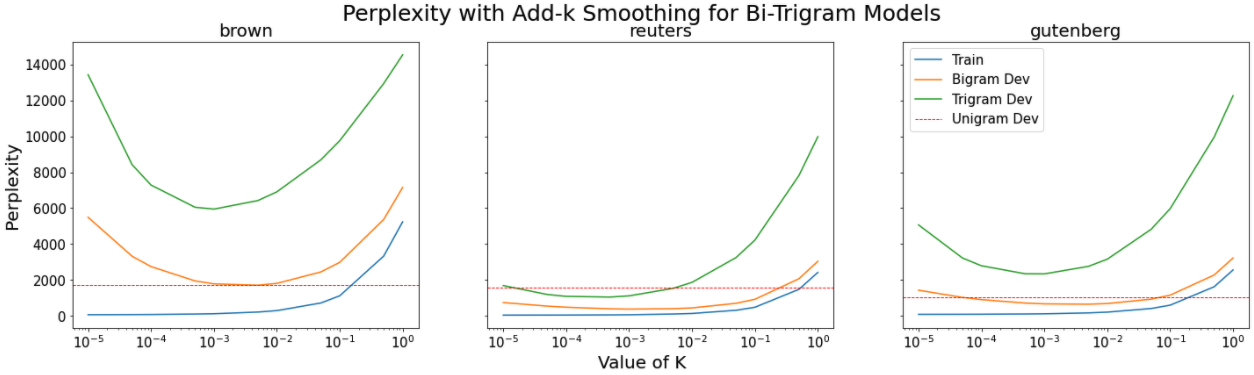
\includegraphics[width=1\linewidth]{imgs/smooth_all.png}
  \caption{Train and dev-set perplexity for bi- and tri-gram 
  language models with vary k in add-k smoothing. A k=1 represents
Laplacian smoothing while dropping k represents weakening the Dirichlet 
prior based on the data. Referenced is dev-set perplexity for unigram models.}
  \label{fig:imgs/smooth_all}
  \vspace{-15pt}
\end{figure*}
\FloatBarrier
%%%%%%%%%%%%%%%%%%%%%%%%%%%%%%%%%%%%%%%%%%%%%%%%%%%%

higher-order n-grams on our performance. Thirdly, we restarted 
this two-step process with stupid backoff smoothing, tuning the n-gram cardinality as well as the
backoff parameter $\lambda$. Other, more sophisticated methods of smoothing including Katz \cite{katz1987estimation}
and Kneser-Ney \cite{kneser1995improved} were not attempted due to time constraints.

%%%%%%%%%%%%%%%%%%%%%%%%%%%%%%%%%%%%%%%%%%%%%%%%%%%%
% Analysis of in and out of domain text
%%%%%%%%%%%%%%%%%%%%%%%%%%%%%%%%%%%%%%%%%%%%%%%%%%%%
\section{Hyperparameter Tuning}%
\label{sec:hyperparam_tuning}

Perhaps the most simple smoothing mechanism for n-gram language models is Laplacian smoothing \cite{mackay1995hierarchical}.
In general, conditional token probabilities given context are derived from frequentist estimates (counts) of instances seen
during training. If a token is not seen with a given context at this time, its probability of occurring at test time is set to zero. 
This is an unreasonable assumption solved by smoothing in general. Laplacian smoothing addresses this by adjusting all count-derived
probabilities to the following:

\begin{equation}
  p_{laplace}(w_i) = \frac{C(w_i, w_{i - 1, \cdots i-n+1}) + k }{C(w_{i - 1, \cdots i-n+1}) + k V}
\end{equation}

where $k$ for Laplacian smoothing is equal to 1 and $V$ refers to the size of the vacabulary.
Another way of thinking of Laplacian smoothing is by converting what was originally
a maximum likelihood estimate into a maximum a-posteriori by adding a Dirichlet prior to the data, defined in this project as a 
categorical distribution. In this context, $k$ represents the strength of the prior. With this change, the behavior for 
modeling a completely unknown token by assigning it a very low but positive probability is the same.



Initial experiments with a Laplacian prior yielded poor results, defined in terms of development (dev) set perplexity. We 
determined this issue to be the result of a prior that was too strong and overpowered the witnessed data, even for a bigram 
model. Figure \ref{fig:imgs/smooth_all} explores the impact of scaling down the strength of our prior, determining that
optimal $k=0.01$ for all datasets. For all data, the transition from underfitting to overfitting as $k$ is decreased is clearly seen.

In addition, Figure \ref{fig:imgs/smooth_all} includes the same ablation conducted on a trigram model. It appears that the 
additional capacity of the trigram led it to overfit more easily, resulting in poor generalization relative to the bigram model.
Interestingly, the optimal add-k smoothing for bigrams only improved the \texttt{brown} slightly from its unigram baseline, while
the other corpuses improves substantially. We believe this is due to the diversity of content in the corpus (poetry, sports, plays, etc.).

Curious on if the tendency for higher-order n-grams to overfit could be resolved with a different method of smoothing, we applied an
implementation of stupid backoff. Stupid (naive) backoff (name defined by authors) \cite{brants2007large} operated by querying an n-gram corpus
for a given context-word pair. If no occurrence exist, then the algorithm conducts the same query, but this time on a lower-order n-gram corpus. 
This iteration continues until a match for the word is found (even if it is a unigram). A heuristic penalty of $\lambda = 0.4$ is applied as a 
multiplier after each backoff iteration to improve generalization and keep the resulting probabilities relatively valid. If the word is never found, 
a very low default probability is returned in the same manner as it is for add-k smoothing.


%%%%%%%%%%%%%%%%%%%%%%%%%%%%%%%%%%%%%%%%%%%%%%%%%%%%
% In-domain Analysis - Empirical
%%%%%%%%%%%%%%%%%%%%%%%%%%%%%%%%%%%%%%%%%%%%%%%%%%%%

\subsection{In-Domain Text Analysis: Empirical}%
\label{sec:in_domain_text_analysis_empirical}

Empirically, we found stupid backoff to work exceedingly well relative to the current best add-k performance. For every corpus, dev set perplexity
dropped substantially. However, the \texttt{brown} corpus again was quick to overfit when higher-order n-gram models were applied to it. Trigram models
%%%%%%%%%%%%%%%%%%%%%%%%%%%%%%%%%%%%%%%%%%%%%%%%%%%%
% Figure of backoff
%%%%%%%%%%%%%%%%%%%%%%%%%%%%%%%%%%%%%%%%%%%%%%%%%%%%
\FloatBarrier
\begin{figure*}[htpb]
  \centering
  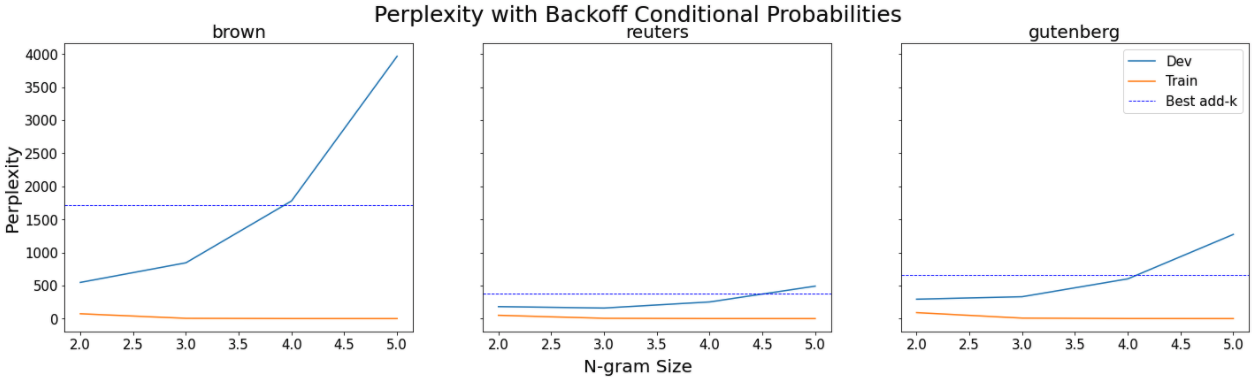
\includegraphics[width=1\linewidth]{imgs/backoff.png}
  \caption{Dev-set perplexity across corpuses with stupid backoff
  smoothing implemented with $\lambda=0.4$ and varing number of
  context sizes (n-gram length). Referenced is current best 
performance from add-k smoothing (dotted).}
  \label{fig:backoff}
  \vspace{-15pt}
\end{figure*}
\FloatBarrier

%%%%%%%%%%%%%%%%%%%%%%%%%%%%%%%%%%%%%%%%%%%%%%%%%%%%


yielded small but notable performance jumps for the other corpuses, but the \texttt{brown} corpus saw a substantial increase in perplexity. Because the
performance jump from bigram to trigram models in the other two corpuses was modest, and with an intention to maximize generalization, we chose a bigram
model implemented with stupid backoff as our tuned model. The baseline unigram performance, along with the performance of our tuned add-k and backoff models
is shown in Table \ref{table:hyperparameter}.


%%%%%%%%%%%%%%%%%%%%%%%%%%%%%%%%%%%%%%%%%%%%%%%%%%%%
% Table for in-domain analysis
%%%%%%%%%%%%%%%%%%%%%%%%%%%%%%%%%%%%%%%%%%%%%%%%%%%%
\begin{table}
\begin{tabular}{llll}
\hline
         & brown       & reuters     & gutenberg   \\
\hline
 uni. & 1514 / 1758 & 1467 / 1577 & 981 / 1036  \\
 add-k   & 128 / 1822  & 72 / 378    & 124 / 650   \\
 b-off & 75 / \textbf{ 559 }    & 51 / \textbf{ 180 }    & 92 / \textbf{ 285 }    \\
\hline
\end{tabular}
\caption{Hyperparameter tuning results. Train and dev-set perplexity across
all three corpuses with different smoothing. add-k and backoff (b-off) 
running optimal k=0.01 and n=2 for ngram models}
\label{table:hyperparameter}
\end{table}

%%%%%%%%%%%%%%%%%%%%%%%%%%%%%%%%%%%%%%%%%%%%%%%%%%%%

Though not shown, varying numbers of $\lambda$ were tested. We found that $\lambda = 0.4$ worked best across all corpuses at
balancing off underfitting (low $\lambda$) and overfitting (high $\lambda$). With our hyperparameter search complete, we 
then explored the behavior of our train bigram models on out of domain data.

%%%%%%%%%%%%%%%%%%%%%%%%%%%%%%%%%%%%%%%%%%%%%%%%%%%%
% Out-of-domain Analysis - Empirical
%%%%%%%%%%%%%%%%%%%%%%%%%%%%%%%%%%%%%%%%%%%%%%%%%%%%

\subsection{Out-of-Domain Text Analysis: Empirical}%
\label{sec:out_domain_text_analysis_empirical}

An insightful way to explore differences between data corpuses is to train a language model on 
one and have it run inference on another. We have conducted this exact experiment below in Table \ref{table:backoff_test_perp} by scoring
the test set perplexity of each language model - corpus pair. As expected, each model determined its own corpus to be the most natural sounding.
More interesting was the similarity between the \texttt{brown} and \texttt{gutenberg} corpuses. The test-set perplexity of the \texttt{gutenberg} 
corpus when evaluated under the \texttt{brown} language model was 841, while \texttt{reuters} was scored over 2100 in the same setting. Furthermore,
When these were evaluated under the \texttt{gutenberg} model, the \texttt{reuters} corpus was seen as four times more perplexing than the \texttt{brown}
corpus. This led us to believe that the lexical characteristic of the \texttt{brown} and \texttt{gutenberg} corpuses were most similar.

%%%%%%%%%%%%%%%%%%%%%%%%%%%%%%%%%%%%%%%%%%%%%%%%%%%%
% Test perplexity for backoff model
%%%%%%%%%%%%%%%%%%%%%%%%%%%%%%%%%%%%%%%%%%%%%%%%%%%%
\begin{table}[h]
\begin{tabular}{lrrr}
\hline
           &   brown &   reuters &   gutenberg \\
\hline
 brown     &  \textbf{ 558.59 } &  2118.33  &     840.811 \\
 reuters   & 1500.02 &   \textbf{ 180.312 } &    2159.68  \\
 gutenberg & 1098.51 &  4240.6   &     \textbf{ 285.342 } \\
\hline
\end{tabular}
\caption{Test set perpexlity for each language model with
  stupid backoff smoothing applied. Each model is applied to 
every corpus.}
\vspace{-10pt}
\label{table:backoff_test_perp}
\end{table}

%%%%%%%%%%%%%%%%%%%%%%%%%%%%%%%%%%%%%%%%%%%%%%%%%%%%

The \texttt{reuters} corpus was also unique for how well its language model could generalize to test data. with a perplexity of 180 it was by far the
most successful in-domain bigram model. We feel this is due to the \texttt{reuters} corpus being domain specific (finance, business) and therefore more
homogenous than the other corpuses. By contrast, the \texttt{brown} corpus was by far the most lexically diverse; its test-set perplexity was over 
3 times higher than the other corpuses and nearly 8 times higher than its train-set perplexity. The difficulty of modeling diverse language for 
downstream tasks is a particularly well explored phenomenon \cite{ponte1998language}. To take a closer look at the differences in these models, 
we feed each model both human and machine generated sentences and observe perplexity scoring a a lower level.



%%%%%%%%%%%%%%%%%%%%%%%%%%%%%%%%%%%%%%%%%%%%%%%%%%%%
% Out-of-domain Analysis - Qualitative
%%%%%%%%%%%%%%%%%%%%%%%%%%%%%%%%%%%%%%%%%%%%%%%%%%%%

\subsection{Qualitative Analysis: Language Scoring}
\label{sub:out_domain_text_analysis_qualitative}



%%%%%%%%%%%%%%%%%%%%%%%%%%%%%%%%%%%%%%%%%%%%%%%%%%%%
% Perplexity findings - scoring of sentences
%%%%%%%%%%%%%%%%%%%%%%%%%%%%%%%%%%%%%%%%%%%%%%%%%%%%
\begin{table}
\begin{tabular}{llll}
\hline
sen. & brown       & reuters     & gutenberg   \\
\hline
  0 & 6836 / 5268 & \textbf{ 490 } / 1571  & 4012 / 6455 \\
  1 & 1901 / 1997 & 1765 / 2670 & \textbf{ 519 } / 1325  \\
  2 & \textbf{ 621 } / 1081  & 5685 / 2628 & 2094 / 1572 \\
  3 & 1011 / \textbf{ 687 }  & 1353 / \textbf{ 1334 } & 1884 / \textbf{ 1473 } \\
 % Generated by gutenberg, most natural under gutenberg
  $4^g$ & 1270 / 1663 & 2296 / 2656 & \textbf{ 124 } / 1271   \\
  % Generated by reuters, most natural under brown, gutenberg
  $5^r$ & \textbf{ 110 } / 335   & 245  / 882   & \textbf{ 111 } / 361   \\
  % Generate by reuters, most natural under reuters
  $6^r$ & 1498 / 2288 & \textbf{ 846 } / 1430  & 3863 / 4466 \\
\hline
\end{tabular}
\caption{Perplexity scoring of sentences (bigram / unigram) (indexed in appendix \ref{table:sentence_reference}) by
  backoff language models. Columns represent the domain of the model used for scoring.
Superscripts denote the domain of the model that generated the sentence, if not human.}
\label{table:sentence_scoring}
\vspace{-15pt}
\end{table}

%%%%%%%%%%%%%%%%%%%%%%%%%%%%%%%%%%%%%%%%%%%%%%%%%%%%

As displayed in Table \ref{table:sentence_scoring}, we have created several sentences (indexed to appendix \ref{table:sentence_reference}) to score 
under our three language models. Sentences 0, 1, and 2 were created by the authors to appear most natural under the   \texttt{reuters},   \texttt{gutenberg}, and \texttt{brown} corpuses, respectively. As expected, the perplexity of our models reflected this intention. Sentence 0, a comment on the financial forecast of Dow Chemical, was given a perplexity score of 490 by the  \texttt{reuters} model, 8x and 10x smaller than the scores given by the \texttt{gutenberg} and \texttt{brown} datasets, respectively. 

By contrast, sentence 1 - a Shakespearean question of resisting temptation - appears most natural under the \texttt{gutenberg} language model, though the contrast between other models is not as stark as sentence 0. Sentence 2, a casual discussion about a football game, was seen as most natural by the \texttt{brown} language model, was seen as nearly 10x more perplexing by \texttt{reuters} but only 3x more perplexing by \texttt{gutenberg}, providing further evidence that the \texttt{brown} and \texttt{gutenberg} corpuses are most similar. Lastly, sentence 3 is most unique because the unigram model for all corpuses scored a lower perplexity. 

A short but modern poetic phrase, sentence 3 seemed most natural under the unigram model because unigrams do not model context. Since all of the words in the phrase are relatively common independently (but not in their present order), n-gram models saw this phrase as unnatural. This demonstrates one of the fundamental challenges of language modeling across domains such as poetry or other literature. The definition of what is a "natural" language phrase is difficult to model holistically. 

Aside from human-generated sentences, we also included three machine generated sentences to compare the \texttt{reuters} and \texttt{guteberg} corpuses. All sentences were seeded with the prefix \texttt{It was like}. Sentence $4^{g}$ was generated by the \texttt{gutenberg} corpus and also categorized as most natural under the same. Sentence $6^{r}$ depicts the same trend for the \texttt{reuters} corpus. Alternatively, $5^{r}$ was generated by the \texttt{reuters} corpus but scored as more natural under the \texttt{brown } and \texttt{gutenberg} corpuses. This is likely due to how short the sentence is; with only a few tokens, the sentence also contains few words that can be solely considered economic terms. These two features together made $5^{r}$ appear unnatural under the domain-specific \texttt{reuters} corpus. We explore this domain specificity in the next section.



%%%%%%%%%%%%%%%%%%%%%%%%%%%%%%%%%%%%%%%%%%%%%%%%%%%%
% Samples of sentences with prefix
%%%%%%%%%%%%%%%%%%%%%%%%%%%%%%%%%%%%%%%%%%%%%%%%%%%%
\rule{0.49\textwidth}{0.4pt}
\label{forecast_ex}
\textbf{Prefix:} \texttt{ \textbf{The forecast} }
\vspace{1mm}

\textbf{Brown:} \texttt{\textbf{The forecast} by an age could flash gangling man found to suppose we have established rapport and payments shall be adjusted Richards of Russia does the at Portsmouth Haverhill and wild}
\vspace{1mm}

\textbf{Reuters:}  \texttt{\textbf{The forecast} on stocks and preferred their trade has led some 11 Pechiney this CBT floor price index has pared severely impair efficiency to elaborate}
\vspace{1mm}

\textbf{Gutenberg:} \texttt{\textbf{The forecast} of Israel 21 say is falleth virtue summon all our servants and his own hands moment they thank them Why did you}

\rule{0.49\textwidth}{0.4pt}
%%%%%%%%%%%%%%%%%%%%%%%%%%%%%%%%%%%%%%%%%%%%%%%%%%%%



%%%%%%%%%%%%%%%%%%%%%%%%%%%%%%%%%%%%%%%%%%%%%%%%%%%%
% Samples of sentences with prefix
%%%%%%%%%%%%%%%%%%%%%%%%%%%%%%%%%%%%%%%%%%%%%%%%%%%%
\rule{0.49\textwidth}{0.4pt}
\label{hath_ex}
\textbf{Prefix:} \texttt{ \textbf{Who hath} }
\vspace{1mm}

\textbf{Brown:}  \texttt{\textbf{Who hath} according to whatever substantial ups unconsciously keeping the could pilots took pride or disquietude he told between eleven at the synergism between 1930}
\vspace{1mm}

\textbf{Reuters:}    \texttt{\textbf{Who hath} QTR NET Shr   28 producing area}
\vspace{1mm}

\textbf{Gutenberg:} \texttt{\textbf{Who hath} failed of up into the man shall hiss What chinn value not your game with thine By at once more in them will Jerusalem saying The mound torrid suns}

\rule{0.49\textwidth}{0.4pt}
%%%%%%%%%%%%%%%%%%%%%%%%%%%%%%%%%%%%%%%%%%%%%%%%%%%%

%%%%%%%%%%%%%%%%%%%%%%%%%%%%%%%%%%%%%%%%%%%%%%%%%%%%
% Language generation
%%%%%%%%%%%%%%%%%%%%%%%%%%%%%%%%%%%%%%%%%%%%%%%%%%%%

\subsection{Qualitative Analysis: Text Generation}
\label{subsec:language_gen}

In our final set of experiments, we qualitatively assess the performance of our language models by seeding them with
several prefixes and observing the output. Shown above in examples \ref{forecast_ex} and \ref{hath_ex}, we seeded sentences with \texttt{The forecast} and \texttt{Who hath}, respectively. Other experiments like this were completed and can be found in our \href{https://github.com/SamShowalter/CS272-NLP/tree/master/hw2}{supporting materials}. We highlight these two prefixes to demonstrate the domain adaptation of our models even when given an out-of-domain prefix. For example, the prefix \texttt{Who hath} originates from old-English that is found in the Gutenberg corpus, forcing the other models to adapt. The \texttt{reuters} model converts this prefix into a question of if someone has shares of stock or assets. Additionally, the sentence also appears most unnatural of all three. The \texttt{brown} corpus does a much better job of generating a natural sentence, but still lacks compared to \texttt{gutenberg} which produced a near-biblical phrase. 

As a comparison, we also fed each model a more general seed of \texttt{The forecast}, one that could yield multiple interpretations. The language models took advantage of this ambiguity to resolve the prefix into its domain. The \texttt{reuters} model discussed the forecast of basic and preferred stocks, \texttt{brown} quoted something that vaguely resembles historical prose, and again \texttt{gutenberg} interprets the forecast as "Israel 21," a pseudo-biblical passage. Though qualitative, the extent to which each generated sentence appears domain specific seems indicative of the lexical homogeniety of the training corpus. From this lense, the \texttt{brown} corpus appears the most linguistically diverse, and \texttt{reuters} the least, mirroring quantitative findings.

Included in appendix \ref{sec:unigram_generated_sentences}, generated sentences from unigram models loosely replicate the findings of our tuned n-gram models, with a few notable exceptions. First, unigram models are poor at conjugating phrases and developing coherent thoughts due to their lack of conditioning on history and sampling from the marginal distributions of words. N-gram models are far better at this even with only single word context (bigrams), though long phrases tend to progressively lose coherence. 


%%%%%%%%%%%%%%%%%%%%%%%%%%%%%%%%%%%%%%%%%%%%%%%%%%%%
% Conclusion
%%%%%%%%%%%%%%%%%%%%%%%%%%%%%%%%%%%%%%%%%%%%%%%%%%%%
\section{Discussion and Conclusion}%
\label{sec:disc_conclusion}

Considered together, our quantitative and qualitative findings yielded several insights. Regarding the \texttt{brown} corpus, we found it surprising that our add-k smoothing struggled to even slightly outperform the unigram baseline compared to the other corpuses. After further examination, we feel this is because this corpus is far more linguistically diverse than its counterparts. This is confirmed by the tendency for language models to overfit to testing data for the \texttt{brown} corpus and the discovery that this corpus includes many different forms of language, from sports to poetry. Even with a more sophisticated smoothing method, stupid backoff, language models struggled to fit well to the data and not overfit \ref{fig:backoff}. 

Most likely, this linguistic diversity was part of the reason why the \texttt{brown} corpus generalized much better to the \texttt{gutenberg} texts than \texttt{reuters}. Full of domain-specific terminology, the \texttt{reuters} corpus was considered an almost completely foreign dialect when viewed from the other models. This observation is partially true, which many terms in the \texttt{reuters} unambiguously financial and business related. Though each corpus observes some domain-specificity (e.g. biblical references and old-English from \texttt{gutenberg} ), the concentration of domain-specific terms is most pronounced in \texttt{reuters}. Evidence of this homogeneity can be seen with the incredibly low perplexity values \texttt{reuters} had on its testing corpus relative to other models. However, this excellent in-domain generalization came at the cost of poor out-of-domain adaptation. 

In a sense, the \texttt{reuters} model intended to capture business-centric phrases more so than English. In \texttt{reuters}-generated phrases that included little business jargon, the \texttt{brown} and \texttt{gutenberg} corpuses scored the statement as more natural. At the same time, it proved nearly impossible to generate a sentence using the \texttt{brown} or \texttt{gutenberg} models that scored a lower perplexity with \texttt{reuters}. Generally, this lends the insight that language models for domain-specific tasks can be improved by training on a subset of only relevant language, but may subsequently struggle to generalize in out-of-domain tasks. In several cases, the in-domain benefit may justify this trade-off.






%%%%%%%%%%%%%%%%%%%%%%%%%%%%%%%%%%%%%%%%%%%%%%%%%%%%

%%%%%%%%%%%%%%%%%%%%%%%%%%%%%%%%%%%%%%%%%%%%%%%%%%%%
% Statement of Collaboration
%%%%%%%%%%%%%%%%%%%%%%%%%%%%%%%%%%%%%%%%%%%%%%%%%%%%
\section{Statement of Collaboration}

I solicited the help of Anthony Chen in asking a few questions about issues I was having with 
my smoothing techniques and the assignment in general. Beyond this discussion and perusing 
Campus Wire, I completed this independently.

%%%%%%%%%%%%%%%%%%%%%%%%%%%%%%%%%%%%%%%%%%%%%%%%%%%%



\bibliography{custom}
\bibliographystyle{acl_natbib}

\appendix
  \label{appendix}

\section{Sentence Reference}%
\label{sec:sentence_ref}

Below is a reference for table with generated sentences. As noted above, the sentences indexed in \ref{table:sentence_scoring} with an additional superscript were generated by the \texttt{reuters} model while $g$ references \texttt{gutenberg}.

\vspace{4mm}
\begin{tabular}{p{0.1\linewidth}|p{0.85\linewidth}}
\hline
   index & sentence                                                                                        \\
\hline
       0 & This third quarter fiscal forecast for DOW Chemical is bearish according to financial analysts. \\
       1 & Who hath such scuples as to remain untrodden by the perils of temptation?                       \\
       2 & Hey did hear about that fight the football team got in to after practice?                       \\
       3 & Walked alone did she, on to tomorrow.                                                           \\
       $4^g$ & It was like fire sent them and new psychological influences set in stone brought the Holy Ghost \\
       $5^r$ & It was like the workforce body                                                                  \\
       $6^r$ & It was like a loss for Bahrain Oman and current residents are packing said company spokesman    \\
\hline
\label{table:sentence_reference}
\end{tabular}


\section{Unigram Generated Sentences}
\label{sec:unigram_generated_sentences}


%%%%%%%%%%%%%%%%%%%%%%%%%%%%%%%%%%%%%%%%%%%%%%%%%%%%
% Samples of sentences with prefix -FORECAST -UNIGRAM
%%%%%%%%%%%%%%%%%%%%%%%%%%%%%%%%%%%%%%%%%%%%%%%%%%%%
\rule{0.49\textwidth}{0.4pt}
\label{forecast_ex_unigram}
\textbf{Prefix:} \texttt{ \textbf{The forecast} }
\vspace{1mm}

\textbf{Brown:}  \texttt{\textbf{The forecast} blanket royalty was least is limited story cases heading present be payments movement its two possible the unmistakably}
\vspace{1mm}

\textbf{Reuters:}    \texttt{\textbf{The forecast} sales late and practices}
\vspace{1mm}

\textbf{Gutenberg:} \texttt{\textbf{The forecast} point blossoms blossoms out won mark is natured incommodiously}

\rule{0.49\textwidth}{0.4pt}
%%%%%%%%%%%%%%%%%%%%%%%%%%%%%%%%%%%%%%%%%%%%%%%%%%%%

%%%%%%%%%%%%%%%%%%%%%%%%%%%%%%%%%%%%%%%%%%%%%%%%%%%
% Samples of sentences with prefix -WHO HATH - UNIGRAM
%%%%%%%%%%%%%%%%%%%%%%%%%%%%%%%%%%%%%%%%%%%%%%%%%%%%
\rule{0.49\textwidth}{0.4pt}
\label{hath_ex_unigram}
\textbf{Prefix:} \texttt{ \textbf{Who hath} }
\vspace{1mm}

\textbf{Brown:} \texttt{\textbf{Who hath} the automatically the efficiency}
\vspace{1mm}


\textbf{Reuters:}   \texttt{\textbf{Who hath} to Ray agency was}
\vspace{1mm}

\textbf{Gutenberg:} \texttt{\textbf{Who hath} said she Till the the at there and the news you and hands mouse shall 28 strength entrance assistants my from}

\rule{0.49\textwidth}{0.4pt}
%%%%%%%%%%%%%%%%%%%%%%%%%%%%%%%%%%%%%%%%%%%%%%%%%%%%

\end{document}% File acl2020.tex

